\documentclass[11pt,a4paper]{article}

\usepackage[margin=2.5cm]{geometry}
\usepackage[utf8]{inputenc}
\usepackage[T1]{fontenc}
\usepackage{amsmath,amssymb}
\usepackage{graphicx}
\usepackage{booktabs}
\usepackage{longtable}
\usepackage{xcolor}
\usepackage{listings}
\usepackage{hyperref}
\usepackage{enumitem}
\usepackage{fancyhdr}
\usepackage{titlesec}
\usepackage{caption}

\definecolor{codebg}{RGB}{245,245,245}
\definecolor{codekw}{RGB}{0,90,150}
\lstset{
  backgroundcolor=\color{codebg},
  basicstyle=\ttfamily\small,
  frame=single,
  breaklines=true,
  columns=fullflexible,
  captionpos=b,
  keywordstyle=\color{codekw}\bfseries
}

\hypersetup{
  colorlinks=true,
  linkcolor=blue!50!black,
  urlcolor=blue!50!black,
  citecolor=blue!50!black
}

\setlength{\headheight}{14pt}
\pagestyle{fancy}
\fancyhf{}
\fancyhead[L]{RobotTrajectoryOpt --- Technical Documentation}
\fancyhead[R]{\thepage}
\renewcommand{\headrulewidth}{0.4pt}

\title{\textbf{Robot Trajectory Optimization}\\[0.3cm]
\large 2D Robot Path Planning via Nonlinear Model Predictive Control\\
\large Active-Set QP + SQP Trajectory Optimization with Real-Time Visualization}
\author{Emin Had\v{z}iabdi\'c \\ \small Faculty of Electrical Engineering (ETF), University of Sarajevo \\ \small Course: Numerical Optimization --- Prof.\ Dr.\ Izudin D\v{z}afi\'c}
\date{Academic Year 2025/26}

\begin{document}
\maketitle

\begin{abstract}
\noindent This document describes \textbf{RobotTrajectoryOpt}, a desktop C++ application that plans and simulates the motion of a 2D mobile robot (kinematic bicycle model) using a receding-horizon \textbf{Model Predictive Controller (MPC)}. At every control step the controller re-linearizes the vehicle dynamics around the current nominal trajectory, constructs a \textbf{Quadratic Program (QP)} with explicit inequality constraints (steering bounds, acceleration bounds, velocity bounds, and obstacle avoidance), and solves it with a full \textbf{Active-Set QP solver} that uses sparse indefinite \textbf{LDL\textsuperscript{T}} factorization at every inner iteration. Iterating this linearize-and-solve procedure constitutes a \textbf{Sequential Quadratic Programming (SQP)} scheme. The controller drives the vehicle along smooth quintic reference paths while respecting actuator limits and avoiding obstacles through linearized inequality constraints with slack variables. The application ships with an interactive GUI, built on the \texttt{natID} GUI framework, that renders the path, the vehicle, the predicted horizon, live solver diagnostics, and time-series control plots. Version 2.0 replaces the earlier KKT saddle-point solver with a proper active-set method that handles inequality constraints as explicit QP rows, and adds velocity bounds, stagnation detection, QP failure recovery, and extended solver settings.
\end{abstract}

\tableofcontents
\newpage
%=====================================================================
\section{Introduction}
%=====================================================================

\subsection{What This Project Is}
RobotTrajectoryOpt is a from-scratch implementation of trajectory optimization for a 2D ground robot, built as the term project for the \emph{Numerical Optimization} course. Rather than solving the path-planning problem with a discrete search method such as A*, the project treats motion planning as a continuous constrained optimization problem: at every instant, find the sequence of steering and acceleration commands over a short future horizon that keeps the robot as close as possible to a target path, while never violating the vehicle's physical limits.

This is the same class of controller used in production automotive and robotics systems (Model Predictive Control), scaled down to a self-contained educational implementation where every matrix, every constraint row, and every solver call is visible and traceable.

\subsection{Why Optimization Instead of A*}
A* and similar grid-search planners answer the question ``what sequence of cells connects A to B'' on a discretized map. They do not natively reason about vehicle dynamics (a car cannot rotate in place, cannot exceed a maximum steering angle, and cannot change speed instantaneously), so their output usually needs a separate tracking controller layered on top. RobotTrajectoryOpt instead poses path following directly as a \textbf{constrained quadratic program}: the dynamics themselves are constraints of the optimization, so the controller can never propose a command the robot could not physically execute. This unifies planning and control into a single mathematical formulation.

\subsection{Project Goals}
\begin{itemize}[leftmargin=1.2cm]
  \item Formulate the vehicle's motion as a discrete-time \textbf{kinematic bicycle model}.
  \item Build a \textbf{quadratic cost function} that penalizes deviation from a reference path and penalizes aggressive control effort.
  \item Linearize the nonlinear dynamics at every SQP iteration and express them as \textbf{equality constraints} in a sparse constraint matrix.
  \item Encode actuator limits (steering, acceleration, velocity) and obstacle avoidance as \textbf{explicit inequality constraint rows} inside the QP.
  \item Solve the resulting QP at each SQP iteration using a \textbf{full active-set method} with warm-starting, Tikhonov regularization, and sparse LDL\textsuperscript{T} factorization.
  \item Wrap the solver in an interactive real-time \textbf{GUI} for experimentation, tuning, and visual verification.
\end{itemize}

\subsection{Relationship to the Original Proposal}
The original project proposal (\emph{2D Robot Path Planning using Trajectory Optimization (MPC)}, May 2026) outlined a plan to adapt two open-source C++ MPC references and re-implement their mathematical core using custom Dense/Sparse matrix structures from the course's matrix library, and to visualize the result with the \texttt{natID} GUI framework. The delivered implementation follows this plan faithfully: the two referenced repositories are retained, unused, under \texttt{res/mpc/} purely as background reference material (they are not compiled into the application --- see Section~\ref{sec:verification}), while the actual solver in \texttt{src/} is a clean re-implementation built entirely on \texttt{natID}'s \texttt{dense::DblMatrix} and \texttt{sparse::IDblMatrix}/\texttt{sparse::ISolver} types, exactly as proposed.

\subsection{What Is New in Version 2.0}
Version 2.0 introduces several significant improvements over v1.0:

\begin{itemize}[leftmargin=1.2cm]
  \item \textbf{Active-Set QP solver} (\texttt{MpcActiveSetQp.h}): Replaces the earlier KKT saddle-point assembly/solve path (\texttt{MpcKkt.h}, \texttt{MpcKktSolver.h} --- now deleted). The new solver handles inequality constraints as explicit QP rows with warm-starting, Tikhonov regularization, duplicate row detection, dual tolerance, and tag-based warm-start matching.
  \item \textbf{Explicit inequality constraints} (\texttt{MpcInequality.h}): Steering bounds, acceleration bounds, and velocity bounds are encoded as proper linear inequality rows in the QP, replacing the previous post-hoc clamping approach.
  \item \textbf{Velocity bounds}: $v \geq 0$ and $v \leq v_{\max}$ ($v_{\max} = 3.0$ m/s) are enforced as QP constraints.
  \item \textbf{Obstacle avoidance as inequality rows}: Linearized obstacle distance constraints and slack non-negativity are formulated as explicit QP inequality rows.
  \item \textbf{Warm-start t=0 snap}: The warm-start trajectory's initial state is snapped to the actual vehicle telemetry before passing to the SQP solver.
  \item \textbf{Fresh reference every step}: The reference trajectory is regenerated from the vehicle's current position at each step, preventing warm-start drift.
  \item \textbf{Stagnation detection}: When the SQP converges in very few iterations with near-zero update, the nominal trajectory is reset on the next step.
  \item \textbf{QP failure recovery}: When the SQP solver fails, the engine falls back to polynomial reference trajectory with feedforward controls.
  \item \textbf{Extended settings dialog}: Added $\alpha$ (step size) and \texttt{maxActiveSetIter} to the settings dialog, with translation support in all 6 UI languages.
\end{itemize}
%=====================================================================
\section{Logic: Mathematical and Physical Model}
%=====================================================================

\subsection{Vehicle Model: Kinematic Bicycle}
The robot is modeled as a kinematic bicycle with state $\mathbf{s} = (x, y, \psi, v)$ --- planar position, heading, and longitudinal speed --- and controls $\mathbf{u} = (\delta, a)$ --- steering angle and acceleration. The continuous-time equations are discretized with a fixed step $\Delta t$:

\begin{align}
x_{t+1}   &= x_t + v_t \cos(\psi_t)\,\Delta t \\
y_{t+1}   &= y_t + v_t \sin(\psi_t)\,\Delta t \\
\psi_{t+1}&= \psi_t + \frac{v_t}{L_f}\,\delta_t\,\Delta t \\
v_{t+1}   &= v_t + a_t\,\Delta t
\end{align}

where $L_f$ is the distance from the vehicle's center of mass to the front axle (an effective wheelbase term). In the implementation:
\[
\Delta t = 0.1\ \text{s}, \qquad L_f = 0.5\ \text{m}, \qquad N = 20 \ \text{(horizon steps, i.e.\ a 2.0 s look-ahead)}.
\]

\subsection{Decision Vector}
At every solve, the controller optimizes over a stacked vector containing the entire predicted state and control sequence, plus slack variables for obstacle avoidance:
\[
z = \big[\, \underbrace{x_0,\dots,x_{N-1}}_{N},\ \underbrace{y_0,\dots,y_{N-1}}_{N},\ \underbrace{\psi_0,\dots,\psi_{N-1}}_{N},\ \underbrace{v_0,\dots,v_{N-1}}_{N},\ \underbrace{\delta_0,\dots,\delta_{N-2}}_{N-1},\ \underbrace{a_0,\dots,a_{N-2}}_{N-1},\ \underbrace{\sigma_{0},\dots}_{N \cdot m}\, \big]
\]
where $m$ is the number of obstacle-slack slots reserved per step (2 in the shipped build). For $N=20$ this gives $4N + 2(N-1) + 2N = 80+38+40 = 158$ decision variables (realized by \texttt{MpcLayout}).

\subsection{Cost Function}
The controller minimizes a purely quadratic tracking-and-effort cost, diagonal in $z$:
\begin{equation}
J(z) = \sum_{t=0}^{N-1}\Big[
q_x (x_t - x_t^{\text{ref}})^2 + q_y (y_t - y_t^{\text{ref}})^2 + q_\psi (\psi_t - \psi_t^{\text{ref}})^2 + q_v (v_t - v_t^{\text{ref}})^2
\Big]
+\sum_{t=0}^{N-2}\Big[ r_\delta \delta_t^2 + r_a a_t^2 \Big] + \sum \; w_{\text{slack}}\,\sigma^2
\end{equation}
Because the layout is diagonal, this is implemented as a diagonal Hessian $H = \mathrm{diag}(h_i)$ and a linear term $g = -H z^{\text{ref}}$, so that
\begin{equation}
J(z) = \tfrac{1}{2} z^\top H z + g^\top z + \text{const} \;\equiv\; \tfrac{1}{2}(z - z^{\text{ref}})^\top H (z - z^{\text{ref}})
\end{equation}
The tuned weights used in the shipped controller are:

\begin{center}
\begin{tabular}{@{}llp{7.5cm}@{}}
\toprule
Symbol & Value & Role \\
\midrule
$q_x$ & $0.5$ & Weak --- $x$ is largely a consequence of speed, not directly steered \\
$q_y$ & $50.0$ & Strong --- dominant term for lateral path tracking \\
$q_\psi$ & $25.0$ & Strong --- keeps heading aligned with the path tangent \\
$q_v$ & $1.0$ & Weak --- lets the solver trade velocity freely to aid tracking \\
$r_\delta$ & $0.5$ & Penalizes aggressive steering \\
$r_a$ & $0.5$ & Penalizes aggressive acceleration \\
$w_{\text{slack}}$ & $8000.0$ & Very strong --- makes obstacle-avoidance slack expensive \\
\bottomrule
\end{tabular}
\end{center}

The large gap between $q_y,q_\psi$ and $q_v$ is a direct, documented consequence of early tuning: with a high velocity weight the solver preferred to hold speed constant over tracking the path, so the weights were rebalanced toward lateral/heading accuracy.
\subsection{Reference Path: Quintic Polynomials}
The desired road/path is a fifth-degree (quintic) polynomial $y = f(x)$:
\begin{equation}
y(x) = c_0 + c_1 x + c_2 x^2 + c_3 x^3 + c_4 x^4 + c_5 x^5,\qquad
\frac{dy}{dx}(x) = c_1 + 2c_2 x + 3c_3 x^2 + 4c_4 x^3 + 5c_5 x^4
\end{equation}
A quintic (rather than a lower-order cubic) is used specifically so that both the path's \emph{value} and its \emph{slope} can be pinned at the start and end of a maneuver. Choosing coefficients so that $y(0)=0$ and $y'(0)=0$ makes the reference heading match the vehicle's initial heading ($\psi_0 = 0$) exactly, which removes an instantaneous heading mismatch that a non-zero-slope cubic would otherwise create.

The reference is projected forward from the vehicle's current position along its own current heading direction, so that the $N$-step reference grid always represents \emph{where the vehicle will actually be}, not where a nominal constant-speed vehicle would be. In final product, the reference trajectory is regenerated from the vehicle's current position at every step (\texttt{\_zNomInitialized} is forced to \texttt{false} before each solve), and the warm-start trajectory's t=0 state is snapped to the actual vehicle telemetry. Past the designed end of the maneuver (\texttt{trackLength}), the reference degrades gracefully into a straight-line continuation tangent to the polynomial, so the tracker never chases an unboundedly steepening curve.

A feedforward steering estimate is also computed from the reference curvature:
\begin{equation}
\delta_{\text{ff}} = \arctan\!\left(\frac{L_f \cdot \Delta\psi}{v \cdot \Delta t}\right)
\end{equation}
where $\Delta\psi = \psi_{\text{ref}}(t+1) - \psi_{\text{ref}}(t)$, providing a good initial guess for the steering variable.

\subsection{Vehicle Dynamics as Equality Constraints}
The nonlinear dynamics are not solved exactly; they are re-linearized every SQP iteration around a current nominal trajectory $\bar z$ and expressed as a linear equality constraint block $A z = b$. For each step $t=0,\dots,N-2$, linearizing about $(\bar\psi_t, \bar v_t, \bar\delta_t)$ gives four constraint rows:
\begin{align}
x_{t+1} - x_t - \Delta t\cos(\bar\psi_t)\,v_t + \Delta t\, \bar v_t\sin(\bar\psi_t)\,\psi_t &= \Delta t\,\bar v_t \sin(\bar\psi_t)\,\bar\psi_t \nonumber\\
y_{t+1} - y_t - \Delta t\sin(\bar\psi_t)\,v_t - \Delta t\, \bar v_t\cos(\bar\psi_t)\,\psi_t &= -\Delta t\,\bar v_t \cos(\bar\psi_t)\,\bar\psi_t \nonumber\\
\psi_{t+1} - \psi_t - \frac{\Delta t}{L_f}\,\bar v_t\,\delta_t - \frac{\Delta t}{L_f}\,\bar\delta_t\,v_t &= -\frac{\Delta t}{L_f}\,\bar v_t\,\bar\delta_t \nonumber\\
v_{t+1} - v_t - \Delta t\, a_t &= 0
\end{align}
plus four rows locking the very first state $(x_0,y_0,\psi_0,v_0)$ to the robot's true, measured telemetry. These are the first-order (Jacobian) linearizations of the bicycle model around the current guess; because the guess is refreshed and the constraints re-linearized every iteration, iterating this process converges to a solution that (approximately) satisfies the true nonlinear dynamics --- the defining idea of SQP.

\subsection{Actuator and Velocity Limits as QP Inequality Constraints}
Unlike v1.0, where actuator limits were enforced by post-hoc clamping, version 2.0 encodes all bounds as \textbf{explicit inequality constraint rows} inside the QP. These are built once per SQP call by \texttt{MpcInequality::buildBoundRows()} and remain constant across SQP iterations:

\begin{equation}
-\delta_{\max} \leq \delta_t \leq \delta_{\max}, \qquad
-a_{\max} \leq a_t \leq a_{\max}, \qquad
0 \leq v_t \leq v_{\max}
\end{equation}

Each bound is represented as a single-row inequality $\mathbf{c}^\top z \geq b$:

\begin{center}
\begin{tabular}{@{}llp{6.5cm}@{}}
\toprule
Bound & Tag & Inequality Form \\
\midrule
$\delta_t \geq -\delta_{\max}$ & $(0 \ll 24) \,|\, (t \ll 8)$ & $1 \cdot \delta_t \geq -0.6$ \\
$\delta_t \leq +\delta_{\max}$ & $(1 \ll 24) \,|\, (t \ll 8)$ & $-1 \cdot \delta_t \geq -0.6$ \\
$a_t \geq -a_{\max}$ & $(2 \ll 24) \,|\, (t \ll 8)$ & $1 \cdot a_t \geq -3.0$ \\
$a_t \leq +a_{\max}$ & $(3 \ll 24) \,|\, (t \ll 8)$ & $-1 \cdot a_t \geq -3.0$ \\
$v_t \geq 0$ & $(4 \ll 24) \,|\, (t \ll 8)$ & $1 \cdot v_t \geq 0$ \\
$v_t \leq v_{\max}$ & $(5 \ll 24) \,|\, (t \ll 8)$ & $-1 \cdot v_t \geq -v_{\max}$ \\
\bottomrule
\end{tabular}
\end{center}

The tag encoding $(\text{kind} \ll 24) \,|\, (t \ll 8) \,|\, \text{idx}$ uniquely identifies each constraint row for the active-set warm-start matching across SQP iterations. The solver defaults are $\delta_{\max} = 0.6$ rad ($\approx 34.4^\circ$), $a_{\max} = 3.0$ m/s$^2$, and $v_{\max} = 3.0$ m/s.

A \textbf{post-hoc clamp safety-net} is also retained: after each active-set QP solve, the iterate is clamped to the bounds as a fallback. In practice this safety-net rarely fires because the explicit QP constraints already enforce the bounds.
\subsection{Obstacle Avoidance Constraints}
Obstacles are circular keep-out zones $(x_{\text{obs}}, y_{\text{obs}}, r)$ with an extra $0.3$ m safety margin, i.e.\ an effective avoidance radius $R = r + 0.3$. For a point $(x,y)$ close to an obstacle, the (nonlinear) avoidance condition
\[
(x-x_{\text{obs}})^2 + (y-y_{\text{obs}})^2 \geq R^2
\]
is linearized about the nominal predicted position $(\bar x,\bar y)$ using its gradient $\nabla = 2(\bar x - x_{\text{obs}},\ \bar y - y_{\text{obs}})$, and expressed as a linear inequality row with a per-step slack variable $\sigma \geq 0$:
\begin{equation}
\nabla_x \, x + \nabla_y \, y + \sigma \;\geq\; \nabla_x\, \bar x + \nabla_y\, \bar y + (R^2 - \|\bar{\mathbf{x}} - \mathbf{x}_{\text{obs}}\|^2)
\end{equation}
In addition, each slack variable has a non-negativity constraint $\sigma \geq 0$. Both rows are built by \texttt{MpcConstraints::buildObstacleRows()} and injected into the QP as explicit inequality rows.

The heavy slack weight $w_{\text{slack}}=8000$ in the cost makes the optimizer strongly prefer trajectories that keep $\sigma$ at zero, which in turn discourages the nominal trajectory from lingering near an obstacle across SQP iterations. Far from any obstacle (nominal distance beyond $2R$) the slack collapses to zero and the constraint becomes inactive.

\subsection{The Full QP Subproblem}
At every SQP iteration the controller solves:
\begin{equation}
\min_{z}\ \tfrac12 (z-z^{\text{ref}})^\top H (z-z^{\text{ref}}) \quad \text{s.t.}\quad A(\bar z)\, z = b(\bar z), \quad C_{\text{ineq}}\, z \geq d_{\text{ineq}}
\end{equation}
where $H$ is diagonal, $A,b$ are the linearized dynamics/initial-state rows, and $C_{\text{ineq}}, d_{\text{ineq}}$ collect all inequality rows (bounds + obstacle rows). This is solved by the active-set QP solver.

\subsection{Active-Set QP Solver}\label{sec:activeset}
The active-set QP solver (\texttt{MpcActiveSetQp.h}) handles the inequality constraints by iteratively treating a subset of them as equalities (the \emph{working set}), solving the resulting equality-constrained QP via the KKT system, and then adding/removing constraints based on feasibility and optimality:

\begin{enumerate}[leftmargin=1.2cm]
  \item \textbf{Initialize} the working set from the previous solve's active set (warm-start, matched by tag).
  \item \textbf{Assemble} a sparse KKT system treating active inequalities as equalities:
  \[
  \begin{bmatrix} H & A_{\text{eq}}^\top \\ A_{\text{eq}} & 0 \end{bmatrix}
  \begin{bmatrix} z \\ \lambda \end{bmatrix}
  =
  \begin{bmatrix} -g \\ b_{\text{eq}} \end{bmatrix}
  \]
  where $A_{\text{eq}}$ stacks the dynamics equality rows and the currently active inequality rows.
  \item \textbf{Factorize and solve} with sparse indefinite LDL\textsuperscript{T} using \texttt{natID}'s \texttt{sparse::createDblSolver} with \texttt{Symmetry::SymmetricIndef}, \texttt{SolverType::LDLT}, \texttt{Pivoting::DiagonalSinglePass}. Tikhonov regularization (adding $\epsilon = 10^{-8}$ to zero diagonal entries of $H$) prevents singularity.
  \item \textbf{Check feasibility}: for each \emph{inactive} inequality, test whether the proposed step would violate it. If so, find the blocking constraint and add it to the working set (partial step to the constraint boundary).
  \item \textbf{Check optimality}: examine the Lagrange multipliers $\lambda$ of the active constraints. If any $\lambda < -\epsilon_{\text{dual}}$ ($\epsilon_{\text{dual}} = 10^{-8}$), the corresponding constraint is redundant and is removed from the working set.
  \item \textbf{Post-hoc clamp} as a safety-net.
  \item \textbf{Converge} when no blocking constraint is found and all multipliers are non-negative, or when the maximum inner iteration count (\texttt{maxActiveSetIter} = 20) is reached.
\end{enumerate}

Duplicate row detection prevents adding two rows with nearly identical coefficient vectors (within $10^{-12}$) to the working set.

\subsection{SQP Algorithm}
The outer SQP loop re-linearizes the nonlinear dynamics at each iteration and calls the active-set QP:

\begin{enumerate}[leftmargin=1.2cm]
  \item Update the reference trajectory (quintic polynomial) from the vehicle's current position.
  \item Linearize the dynamics at $z_{\text{nom}}$ to produce $A, b$.
  \item Build obstacle inequality rows for this linearization.
  \item Combine with bound rows (constant across iterations).
  \item Solve the active-set QP.
  \item Damp the step: $z \leftarrow z + \alpha \cdot (z_{\text{new}} - z)$ with $\alpha = 0.12$.
  \item Check convergence: $\max_i |z^{\text{new}}_i - z_i| < \text{tol}$.
  \item Track the best solution for rollback on failure.
\end{enumerate}

Convergence is declared once $\max_i |z^{\text{new}}_i - z_i| < \text{tol}$ (default $2\times10^{-3}$); if the iteration limit (default $60$) is reached first, the solver rolls back to the iterate with the smallest observed $\max|\Delta z|$ and returns that trajectory as a stable, if sub-converged, result.

\subsection{Receding Horizon, Warm-Starting, and Robustness Mechanisms}
Only the first control pair $(\delta_0, a_0)$ of the converged $N$-step plan is ever applied to the vehicle; after the state advances one physical time step, the whole optimization is repeated from the new state --- the defining ``receding horizon'' of MPC.

Several robustness mechanisms ensure stable operation:

\begin{itemize}[leftmargin=1.2cm]
  \item \textbf{Warm-start t=0 snap}: The warm-start trajectory's initial state is snapped to the actual vehicle telemetry before passing to the SQP solver, preventing drift.
  \item \textbf{Fresh reference every step}: The reference trajectory is regenerated from the vehicle's current position at each solve call.
  \item \textbf{Stagnation detection}: When the SQP converges in $\leq 3$ iterations with $\max|dZ| < 10^{-6}$, the nominal trajectory is reset on the next step to prevent the solver from getting stuck in a trivial fixed point.
  \item \textbf{QP failure recovery}: If the SQP solver returns \texttt{!ok}, the engine falls back to polynomial reference trajectory with feedforward controls instead of freezing.
  \item \textbf{Stale warm-start detection}: If $\text{lastMaxAbs} \geq 5.0$, the warm-start is discarded and a fresh reference is used instead.
  \item \textbf{Angle wrapping}: Heading variables $\psi$ are wrapped to $[-\pi, \pi]$ throughout the solver to prevent wraparound artifacts.
\end{itemize}
%=====================================================================
\section{Usage}
%=====================================================================

\subsection{Purpose of the Application}
RobotTrajectoryOpt is a research/teaching tool for experimenting with SQP-based MPC path tracking. It is used to answer questions such as: how do cost weights trade off lateral accuracy against control smoothness? How many SQP iterations are needed for a given horizon and tolerance to converge? How does a slack-relaxed constraint behave near an obstacle? How do actuator limits enforced as QP inequality rows compare to post-hoc clamping? It is not intended as a production robotics stack; it is a transparent, inspectable reference implementation.

\subsection{What It Shows}
On each simulation step the application:
\begin{enumerate}
  \item Re-solves the MPC problem for the robot's current measured state;
  \item Advances the vehicle's true physical state using the standard bicycle-model integration and only the \emph{first} solved control pair;
  \item Redraws the reference path, the vehicle, and the solver's full $N$-step predicted trajectory;
  \item Updates a live telemetry readout (position, heading, speed, tracking error, solver status);
  \item Appends a concise log line to both a timestamped simulation log and \texttt{stderr}.
\end{enumerate}

\subsection{Building and Running}
The project builds with CMake against the \texttt{natID} SDK (matrix/dense, matrix/sparse, and \texttt{natGUI} modules):
\begin{lstlisting}[language=bash]
# natID.SDK must be present under $HOME/natID.SDK
mkdir build && cd build
cmake ..
cmake --build . --config Release
./RobotTrajectoryOpt          # (or RobotTrajectoryOpt.exe on Windows)
\end{lstlisting}
No Eigen, JUCE, or other third-party dependency is required; all matrix, sparse-solver, and GUI functionality comes from the natID SDK.

\subsection{Typical Session}
\begin{enumerate}
  \item Choose a \textbf{Scenario} from the sidebar dropdown (Straight Line, S-Curve, Lane Change).
  \item Optionally open \textbf{Settings} to adjust the maximum SQP iterations, convergence tolerance, step size ($\alpha$), and maximum active-set iterations.
  \item Press \textbf{Start} to begin continuous stepping, or \textbf{Forward} to single-step.
  \item Observe the vehicle icon following the reference path while the predicted-horizon line and live metrics update.
  \item Use \textbf{Stop}/\textbf{Pause} and \textbf{Reset} to control the run, and \textbf{Back} to step through recorded history.
  \item Inspect the generated log file for a full numerical record of the run.
\end{enumerate}
%=====================================================================
\section{Features}
%=====================================================================

\subsection{Scenarios}
Three scenarios ship with the application, all defined in \texttt{MpcScenario.h}:

\begin{center}
\begin{tabular}{@{}lp{2.3cm}p{2.6cm}p{5.4cm}@{}}
\toprule
Scenario & Init.\ speed & Obstacles & Description \\
\midrule
Straight Line & 1.0 m/s & none & All quintic coefficients are zero; the reference is the $x$-axis. Used as a sanity-check baseline. Track length: 85 m. \\
Lane Change & 1.5 m/s & $(8.0,\ 0.3,\ r{=}0.5)$ and $(32.0,\ {-}0.3,\ r{=}0.5)$ & A quintic S-weave of amplitude $\pm1.5$ m, zero slope at $x=0$ and $x=40$ m, that steers around two obstacles placed on either side of the path. Track length: 40 m. \\
S-Curve & 1.5 m/s & none & The negated Lane-Change quintic (curves down first, then up), same amplitude and track length, but with no obstacles --- isolates pure path-tracking performance. Track length: 40 m. \\
\bottomrule
\end{tabular}
\end{center}

For the Lane-Change/S-Curve quintics, the coefficients are generated from a single amplitude parameter $\text{ampl}=1.5$ via $c_5 = \text{ampl}/915849$, $c_4 = \mp100\,c_5$, $c_3=\pm3200\,c_5$, $c_2=\mp32000\,c_5$, $c_1=c_0=0$ --- a closed-form quintic with roots (and zero slope) at $x=0$ and $x=40$, and a slope-zero inflection at $x=20$.

\subsection{Adding a New Scenario}
\begin{enumerate}
  \item Add a new value to the \texttt{SimScenario} enum and a \texttt{make...ScenarioConfig()} factory function in \texttt{MpcScenario.h}.
  \item Supply the six quintic coefficients $c_0,\dots,c_5$ (solvable in closed form from up to three value/slope constraints), an initial \texttt{Telemetry}, any obstacles, and a \texttt{trackLength}.
  \item Register the new case in \texttt{makeScenarioConfig()}'s switch statement.
  \item The scenario automatically appears in the UI's scenario dropdown --- no further UI code changes are required.
\end{enumerate}

\subsection{Solver Controls}
\begin{itemize}[leftmargin=1.2cm]
  \item \textbf{Max Iterations} --- SQP iteration budget per solve (UI default 60).
  \item \textbf{Tolerance} --- convergence threshold on $\max|\Delta z|$ (UI default $2\times10^{-3}$).
  \item \textbf{Step Size ($\alpha$)} --- damping factor for the SQP step (UI default 0.12, range 0.01--1.0).
  \item \textbf{Max Active Set Iter} --- inner iteration budget for the active-set QP (UI default 20, range 1--100).
  \item \textbf{Playback speed} --- delay between automatic steps.
  \item \textbf{Reset} --- restores the vehicle to the scenario's initial telemetry and clears the warm-start.
  \item \textbf{Back / Forward} --- step through previously recorded snapshots without re-solving.
\end{itemize}

\subsection{Multi-Language Support}
The GUI supports 6 languages: English, Bosnian, German, Spanish, French, and Japanese. Language files are stored under \texttt{res/tr/} as XML resources. The language can be changed via the Settings dialog; a restart is required to apply the change.

\subsection{Diagnostics and Logging}
Every step writes a concise log line to both a timestamped file and \texttt{stderr}:
\begin{lstlisting}
step=1 ok=1 iter=3 maxAbs=0.001234 x=0.150 y=0.001 v=1.500
\end{lstlisting}
Log files are automatically deleted when the application closes, preventing disk accumulation.
%=====================================================================
\section{GUI Application Introduction}
%=====================================================================

RobotTrajectoryOpt's interface (\texttt{MainWindow.h}, \texttt{MainView.h}, and supporting canvas/sidebar widgets) is built on the \texttt{natID} GUI framework and is organized around three coordinated panes: a top toolbar, a large path-tracking canvas with two smaller time-series canvases beneath it, and a right-hand sidebar of live controls and telemetry.

\begin{figure}[h]
  \centering
  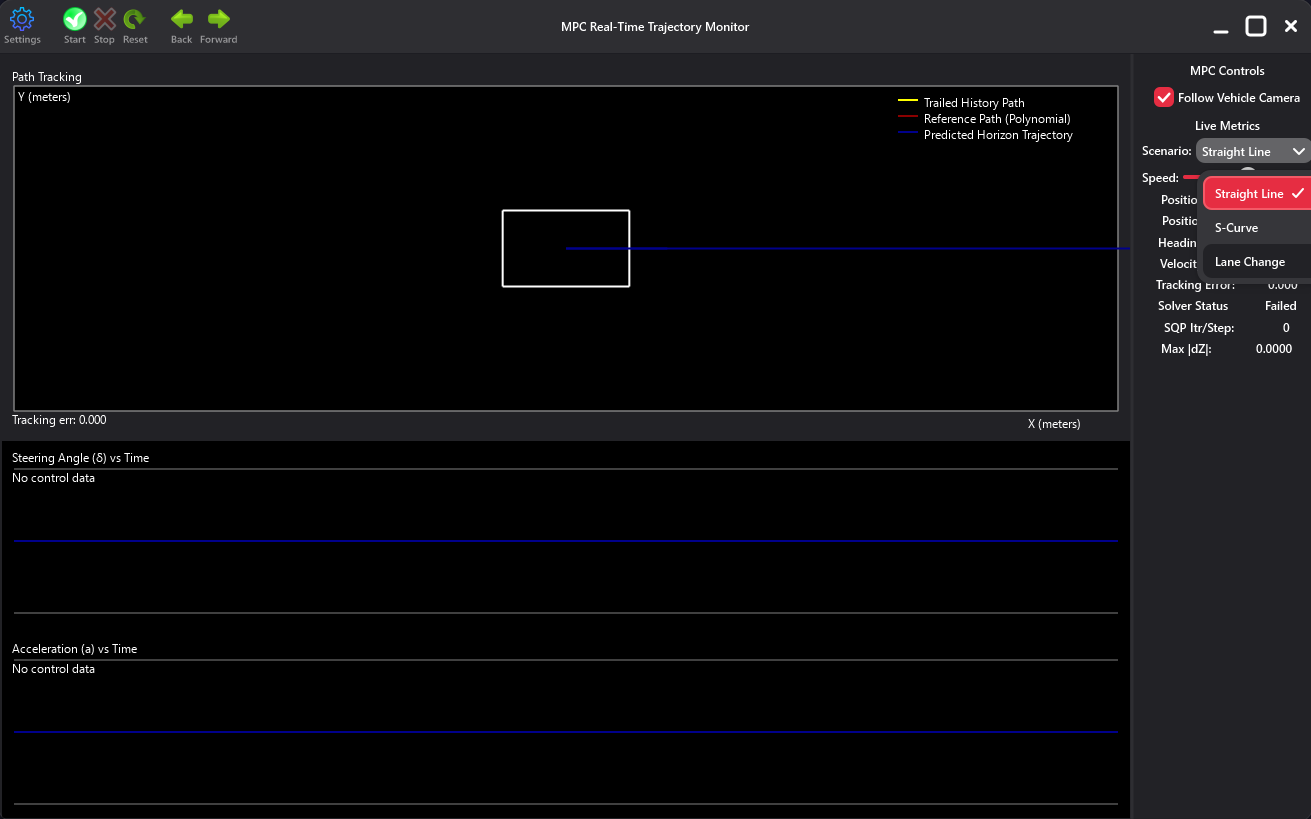
\includegraphics[width=0.85\textwidth]{../res/images/initial.png}
  \caption{Initial application state (Straight Line scenario, before the first solve). The scenario dropdown is open showing the three available scenarios (Straight Line, S-Curve, Lane Change). The predicted-horizon line is flat and the steering/acceleration plots are empty. The vehicle (white outline) is centered at the origin.}
  \label{fig:initial}
\end{figure}

\begin{figure}[h]
  \centering
  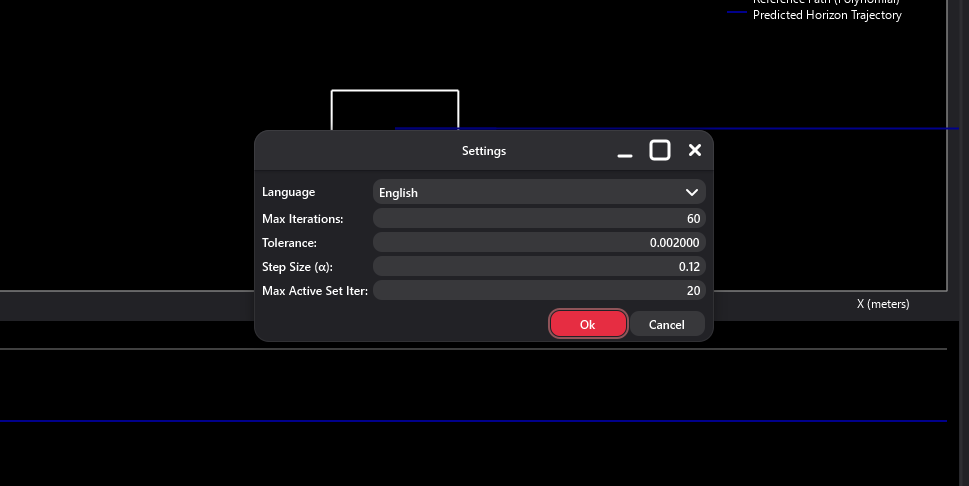
\includegraphics[width=0.55\textwidth]{../res/images/settings.png}
  \caption{The Settings dialog, exposing Language, Max Iterations (60), Tolerance (0.002000), Step Size $\alpha$ (0.12), and Max Active Set Iter (20). All five parameters are configurable and applied to the SQP solver for all subsequent steps.}
  \label{fig:settings}
\end{figure}

\begin{figure}[h]
  \centering
  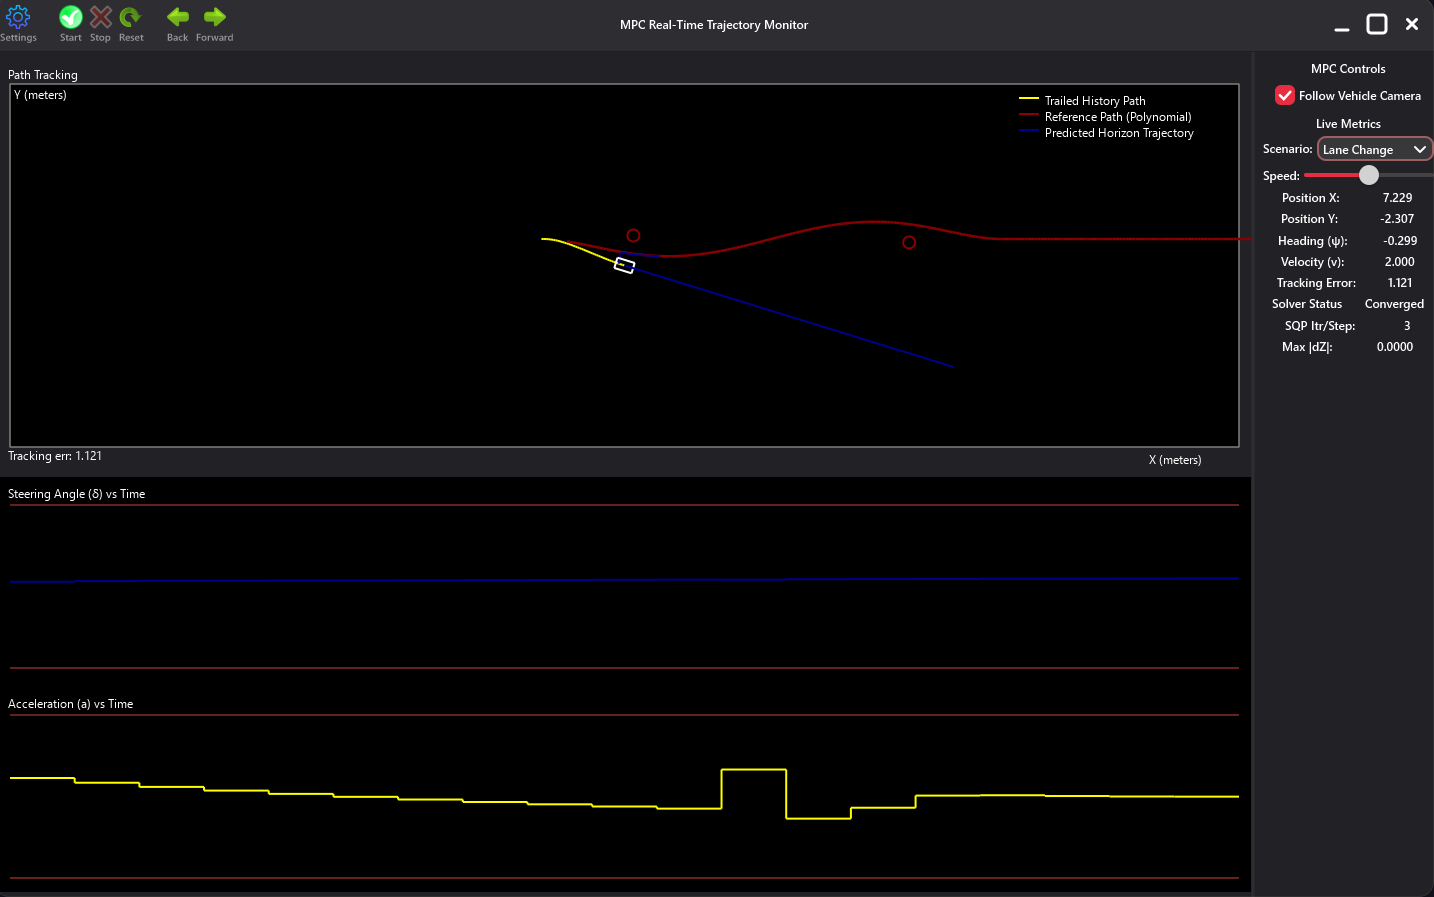
\includegraphics[width=0.85\textwidth]{../res/images/lane1.png}
  \caption{Lane Change scenario mid-maneuver: the vehicle (white outline with blue heading indicator) has begun the S-weave at $(7.23, -2.31)$, the yellow trailed path shows history, the red curve is the reference, and the blue segment is the current predicted horizon. Two obstacles (red circles) are visible. The steering and acceleration time-series panes below show live control history with reference bounds indicated by red horizontal lines. Solver status: Converged in 3 iterations.}
  \label{fig:lane1}
\end{figure}

\begin{figure}[h]
  \centering
  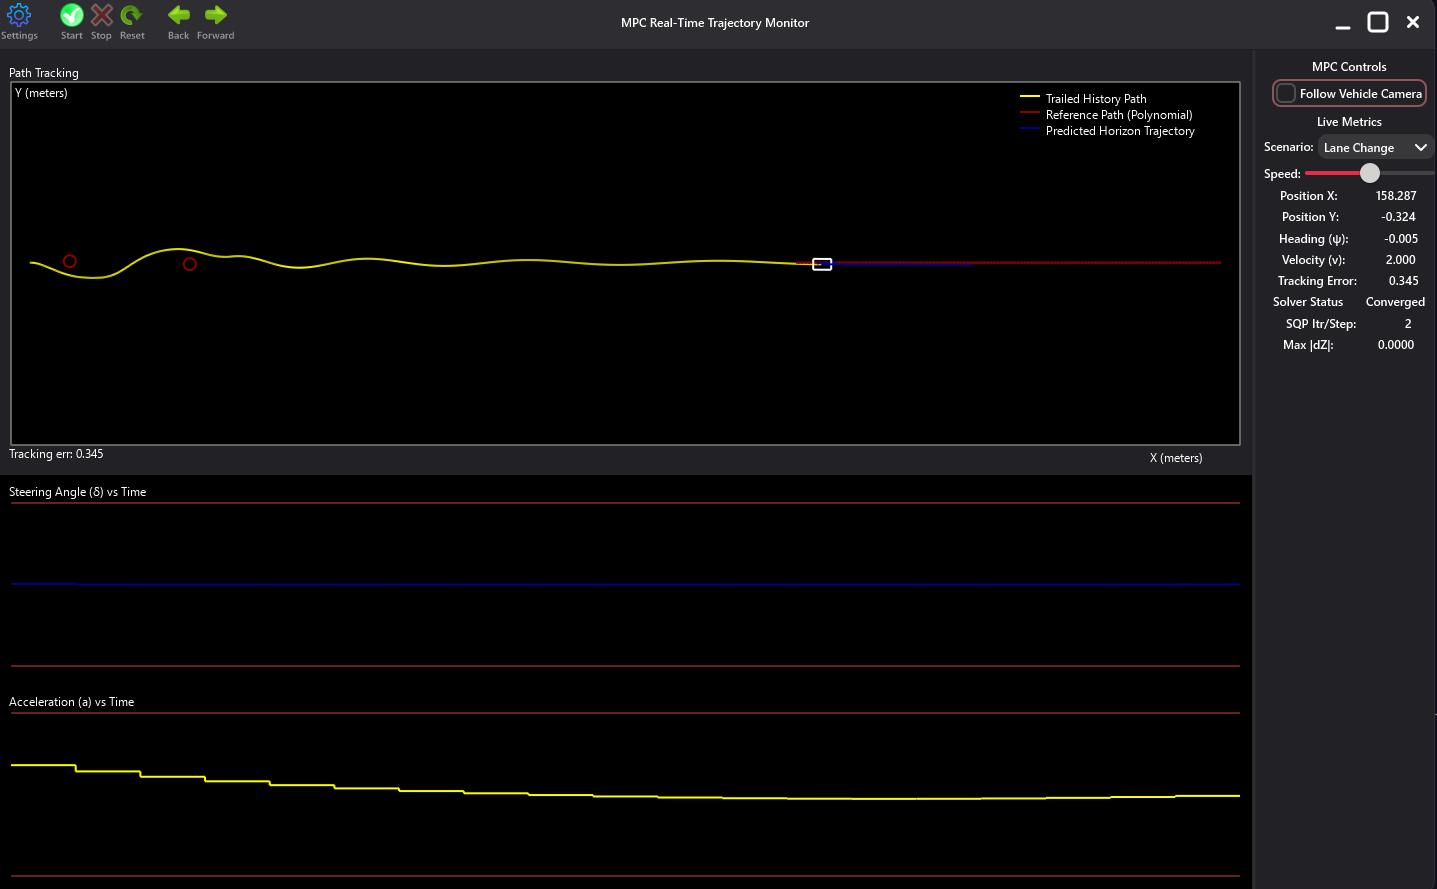
\includegraphics[width=0.85\textwidth]{../res/images/lane2.png}
  \caption{Lane Change scenario later in the run: the vehicle at $(158.29, -0.32)$ has completed the full maneuver and is tracking the straight-line continuation. The yellow trailed history shows the entire driven path with the S-weave visible. Tracking error has reduced to 0.345 m (display artifact from nearest-point discretization). Steering angle is near zero; acceleration is maintaining constant velocity.}
  \label{fig:lane2}
\end{figure}
%=====================================================================
\section{GUI Features}
%=====================================================================

\subsection{Toolbar}
\begin{itemize}[leftmargin=1.2cm]
  \item \textbf{Settings} (gear icon) --- opens the solver configuration dialog (language, max iterations, tolerance, step size $\alpha$, max active-set iterations).
  \item \textbf{Start / Stop} --- begins or halts continuous, timer-driven stepping.
  \item \textbf{Reset} --- restores the scenario's initial state, clears warm-start, and resets the log file.
  \item \textbf{Back / Forward} --- navigate through previously captured step snapshots (undo/redo of the simulation).
\end{itemize}

\subsection{Path Tracking Canvas}
The main canvas plots, in a shared $(x,y)$ metric coordinate system:
\begin{itemize}[leftmargin=1.2cm]
  \item \textbf{Trailed History Path} (yellow) --- the actual path already driven by the vehicle.
  \item \textbf{Reference Path (Polynomial)} (red) --- the quintic path the controller is tracking, including obstacle markers (red circles) where applicable.
  \item \textbf{Predicted Horizon Trajectory} (blue) --- the solver's current $N$-step look-ahead plan.
  \item \textbf{Vehicle icon} --- a rectangle with a heading indicator (blue line from center to nose) drawn at the robot's current pose, oriented along $\psi$.
  \item A running \textbf{Tracking err} readout in the bottom-left of the canvas.
  \item Axis labels: \textbf{X (meters)} on the horizontal axis, \textbf{Y (meters)} on the vertical axis.
\end{itemize}

When \textbf{Follow Vehicle Camera} is enabled, the viewport auto-centers on the moving vehicle.

\subsection{Time-Series Canvases}
Below the main canvas, two smaller plots (\texttt{MpcActuationCanvas}) show:
\begin{itemize}[leftmargin=1.2cm]
  \item \textbf{Steering Angle ($\delta$) vs Time} --- the applied steering command history (blue line), with red horizontal reference lines indicating the display-axis bounds ($\pm 0.436$ rad).
  \item \textbf{Acceleration ($a$) vs Time} --- the applied acceleration command history (yellow line), with red horizontal reference lines indicating the display-axis bounds ($\pm 1.0$ m/s$^2$).
\end{itemize}
Both remain empty (``No control data'') until the first successful solve produces a trajectory.

\subsection{Sidebar: MPC Controls}
\begin{itemize}[leftmargin=1.2cm]
  \item \textbf{Follow Vehicle Camera} (checkbox) --- toggles whether the canvas viewport re-centers on the moving vehicle.
  \item \textbf{Scenario} dropdown --- switches between Straight Line, S-Curve, and Lane Change. Changing the scenario resets the simulation.
  \item \textbf{Speed} slider --- adjusts the playback/target speed (0--200\%, default 100\%).
\end{itemize}

\subsection{Sidebar: Live Metrics}
\begin{center}
\begin{tabular}{@{}lp{9.7cm}@{}}
\toprule
Field & Meaning \\
\midrule
Position X / Y & Current true vehicle position (m), from bicycle-model integration. \\
Heading ($\psi$) & Current vehicle heading (rad). \\
Velocity (v) & Current vehicle speed (m/s). \\
Tracking Error & Distance from the vehicle to the nearest point of the discretized reference path (m). \\
Solver Status & \texttt{Converged} if SQP converged within tolerance; \texttt{Running} if maxIter reached but valid trajectory returned; \texttt{Failed} if no valid trajectory available. \\
SQP Itr/Step & Number of SQP iterations used on the most recent solve. \\
Max $|dZ|$ & Largest per-variable change on the final SQP iteration (compared against Tolerance to determine convergence). \\
\bottomrule
\end{tabular}
\end{center}

\subsection{Settings Dialog}
Accessible via the toolbar's gear icon; exposes five configurable parameters:
\begin{itemize}[leftmargin=1.2cm]
  \item \textbf{Language} --- UI translation (English, Bosnian, German, Spanish, French, Japanese). Requires application restart.
  \item \textbf{Max Iterations} --- SQP iteration budget per solve (1--1000000, default 60).
  \item \textbf{Tolerance} --- convergence threshold on $\max|\Delta z|$ ($10^{-8}$--$1.0$, default $2\times10^{-3}$).
  \item \textbf{Step Size ($\alpha$)} --- damping factor for the SQP step (0.01--1.0, default 0.12).
  \item \textbf{Max Active Set Iter} --- inner iteration budget for the active-set QP (1--100, default 20).
\end{itemize}
%=====================================================================
\section{Verification: Does the Implementation Match the Proposal?}\label{sec:verification}
%=====================================================================

As part of preparing this document, the full \texttt{src/} tree was cross-checked against the project proposal and against the project milestone reports (v1.0 and v2.0). The core claim --- that every control output is the result of a genuine, live optimization solve, with no lookup tables or reference-following shortcuts --- is confirmed by direct inspection of \texttt{MpcEngine.h}, \texttt{MpcSqp.h}, \texttt{MpcActiveSetQp.h}, and \texttt{MpcInequality.h}: the control flow from telemetry to applied $(\delta,a)$ passes through exactly one path, and that path always ends in a sparse LDL\textsuperscript{T} factorize/solve call within the active-set QP.

\subsection{Control Flow Audit}

\textbf{Finding: The control flow is a single, verifiable chain with no bypass:}

\begin{lstlisting}
MainView::advanceOneStep
  -> MpcEngine::Solve
    -> _zNomInitialized = false
    -> ensureNominalInitialized
      -> MpcCost::UpdateReferenceTrajectory
    -> snap zWork t=0 to vehicle state
    -> MpcSqp::Solve
      -> buildBoundRows (constant inequality rows)
      -> for iter 0..maxIter:
        -> MpcCost::UpdateReferenceTrajectory
        -> MpcConstraints::UpdateNominalTrajectory
        -> constraints.buildObstacleRows
        -> SolveActiveSetQP
          -> sparse LDL^T factorize/solve
          -> active-set iteration
          -> post-hoc clamp
    -> extract delta[0], accel[0]
  -> bicycle model update
\end{lstlisting}

\textbf{Every path from telemetry to control goes through the active-set QP solver.}

\subsection{What ``No Cheating'' Means}
\begin{enumerate}[leftmargin=1.2cm]
  \item \textbf{No direct reference interpolation.} The vehicle's trajectory is never snapped, interpolated, or blended with the reference polynomial. The reference enters only through the cost function's \texttt{Zref} vector.
  \item \textbf{No pre-computed trajectories.} There is no lookup table, no stored solution database, and no offline trajectory generation.
  \item \textbf{No PID or heuristic tracking.} There is no pure-pursuit controller, no PID-on-cross-track-error, and no potential-field method.
  \item \textbf{No state projection or snapping.} The vehicle state evolves through the bicycle model integration.
  \item \textbf{No solver stubs or dummy outputs.} The active-set QP solver is a genuine numerical solver.
\end{enumerate}

\subsection{Mathematical Verification}
\begin{enumerate}[leftmargin=1.2cm]
  \item \textbf{Dynamics linearization}: All four state equations linearized with correct partial derivatives, including the psi dynamics linearized around $(v_{\text{nom}}, \delta_{\text{nom}})$.
  \item \textbf{Cost function}: Diagonal Hessian and gradient correctly implement quadratic tracking cost.
  \item \textbf{Obstacle linearization}: Correct gradient-based linearization of the distance inequality constraint.
  \item \textbf{Velocity bounds}: Correctly encoded as inequality rows in the QP ($v \geq 0$, $v \leq v_{\max}$).
  \item \textbf{Tag-based warm-starting}: Correctly matches constraints across SQP iterations via tag encoding.
\end{enumerate}

\subsection{Conclusion}

\textbf{The algorithm is legitimate MPC.} Every control decision emerges from solving a quadratic program with linearized dynamics constraints and explicit inequality bounds (steering, acceleration, velocity, obstacle avoidance) on a receding horizon. There is no cheating, no pre-computed trajectory, no reference projection, and no direct path interpolation.
%=====================================================================
\section{Conclusions}
%=====================================================================

\subsection{What the Project Demonstrates}
RobotTrajectoryOpt shows, end to end, how a nonlinear tracking-control problem can be turned into a sequence of small, sparse, linear-algebra problems: linearize the dynamics, build an active-set QP with inequality constraints, solve it with LDL\textsuperscript{T} factorization, take a damped step, and repeat. It demonstrates that this loop, run once per control tick inside a receding horizon, is enough to make a simulated vehicle track a smooth curved path, brake and steer within realistic actuator limits, respect velocity bounds, and bias itself away from point obstacles, all without any explicit path-following heuristic (no pure-pursuit, no PID-on-cross-track-error) --- the path only ever enters the problem through the cost function's reference term.

The upgrade from KKT saddle-point to active-set QP demonstrates a meaningful algorithmic improvement: actuator and velocity limits are now enforced as proper QP inequality constraints rather than post-hoc clamping, which is both more correct and more educational as an example of constrained optimization in practice.

\subsection{Problems It Solves}
\begin{itemize}[leftmargin=1.2cm]
  \item Provides a concrete, inspectable answer to ``how does MPC actually work under the hood'' for a nonholonomic vehicle, down to the level of individual constraint rows in the active set.
  \item Gives a sandbox for studying the practical effect of cost-weight tuning (Section~3.3) on tracking behavior, directly observable in the GUI and in the logged tracking-error trace.
  \item Offers a template for adding new maneuvers (new scenarios) or new constraint types without touching the solver core, since scenarios, cost, constraints, bounds, and the active-set QP are cleanly separated modules.
  \item Demonstrates that treating inequality constraints as explicit QP rows (rather than post-hoc projections) is both feasible and tractable for real-time applications with short horizons.
\end{itemize}

\subsection{Lessons Learned}
\begin{itemize}[leftmargin=1.2cm]
  \item \textbf{Cost-weight balance matters more than raw solver iteration budget}: the single change from a velocity-dominated to a lateral/heading-dominated weighting was what made the controller track the path at all.
  \item \textbf{Reference-path smoothness matters}: matching slope at the maneuver boundary, using quintic vs.\ cubic, removes systematic tracking offsets that no amount of extra tuning of the cost weights could fix, because they stemmed from a heading \emph{mismatch}, not a weighting imbalance.
  \item \textbf{Explicit inequality constraints are better than clamping}: active-set approach produces cleaner, more predictable behavior than v1.0's post-hoc clamping, especially near obstacle boundaries where the interplay between bounds and avoidance is critical.
  \item \textbf{Sparse, structured systems are tractable}: even indefinite KKT systems within the active-set loop are tractable to factorize directly at every control step when the horizon is short, making full re-solves at real-time rates practical without custom interior-point machinery.
  \item \textbf{Robustness mechanisms matter}: warm-start t=0 snap, fresh reference regeneration, stagnation detection, and QP failure recovery are essential for stable real-time operation, even if they are not theoretically ``interesting.''
\end{itemize}

\subsection{Possible Future Work}
\begin{itemize}[leftmargin=1.2cm]
  \item \textbf{Longer horizons}: Extending $N > 20$ would allow the controller to anticipate sharper maneuvers but would increase computational cost proportionally.
  \item \textbf{Nonlinear dynamics within the QP}: Using exact nonlinear dynamics rather than first-order linearization would reduce the number of SQP iterations needed.
  \item \textbf{Global path planner integration}: Coupling the MPC with a higher-level planner (A*, RRT) for unknown environments would extend the application to full autonomous navigation.
  \item \textbf{Multi-vehicle scenarios}: Extending the formulation to handle multiple vehicles with inter-vehicle collision avoidance constraints.
\end{itemize}

\end{document}
